\documentclass[12pt]{article}
\usepackage{graphicx} %package to manage images
\graphicspath{ {./figures/} }
\usepackage{caption}
\usepackage[font=scriptsize]{subcaption}
\captionsetup[figure]{labelsep=none}
\captionsetup[table]{labelsep=none}
\usepackage{bbm}
\usepackage{amsmath}
\usepackage{import}
\usepackage{array}
\usepackage{booktabs}
\usepackage{afterpage}
\usepackage{floatrow}
\usepackage{pdflscape}
\usepackage{soul}
\usepackage{float}
\usepackage{adjustbox}
\usepackage{longtable}
\usepackage{caption}
\usepackage{setspace}
\usepackage{afterpage}
\usepackage[margin=1in]{geometry}
\usepackage[round]{natbib}
\usepackage{hyperref}
\usepackage{titlesec}

\title{EGC Stata Test 070625 S278}
\author{Sidh Pandit}
\date{August 2025}

\begin{document}

\maketitle


\subsection{part c}

\begin{table}[H]
    \centering
    \scriptsize % shrink text
    \setlength{\tabcolsep}{2pt}
    \renewcommand{\arraystretch}{2}
    \resizebox{\textwidth}{!}{{
\def\sym#1{\ifmmode^{#1}\else\(^{#1}\)\fi}
\begin{tabular}{l*{3}{cccccc}}
\hline\hline
            &\multicolumn{6}{c}{hhinc\_topcoded}                                           &\multicolumn{6}{c}{log\_hhinc\_topcoded}                                       &\multicolumn{6}{c}{log\_hhinc\_topcoded}                                       \\
            &        Mean&          SD&   1st pctl.&      Median&  99th pctl.&         Max&        Mean&          SD&   1st pctl.&      Median&  99th pctl.&         Max&        Mean&          SD&   1st pctl.&      Median&  99th pctl.&         Max\\
\hline
\hline
\(N\)       &        4160&            &            &            &            &            &        3916&            &            &            &            &            &        3584&            &            &            &            &            \\
\hline\hline
\multicolumn{19}{l}{\footnotesize 24-month income is estimated by 24*household income in last 30 days.}\\
\end{tabular}
}
}
    \caption{: Endline raw data summary statistics}
\end{table}

The average household in this sample earns 11,809 Rs. per month, with an average of 4.51 household members. This translates to a per-capita daily income of approximately 89.42 Rs., or 6.29 USD per day using the provided exchange rate. Though this average was well above the international threshold for extreme poverty at the time, it masks stark inequalities.

The median household income is 6,000 Rs., nearly half the mean, suggesting that most households live on modest incomes while a smaller minority earn largely more.

Among the sample, borrowing is substantial with households having on average total formal loans of 64,382 Rs. and informal loans of 40,921 Rs., though these distributions are also skewed right and influenced by extreme upper outliers. 

Nonetheless, the amount of informal borrowing may suggests possible financial exclusion among the sample, strong informal credit networks, or a preference for informal borrowing.


\begin{figure}[H]
    \centering
    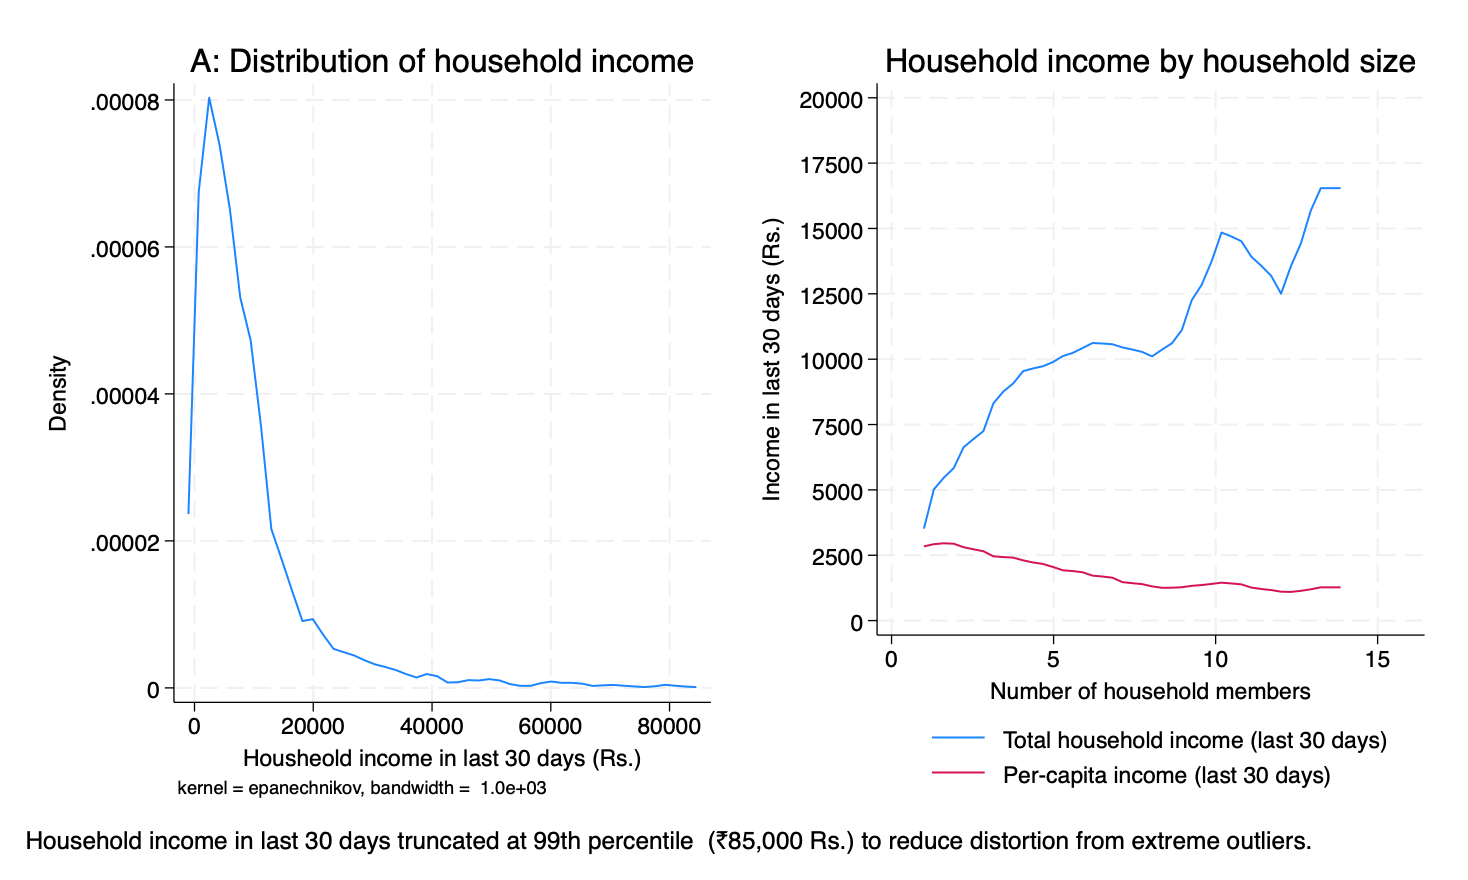
\includegraphics[width=\textwidth]{figures/figure01_hhinc.png}
    \caption{: Distribution and composition of household income in last 30 days}
\end{figure}

Panel A visually confirms the skewed distribution even after excluding the top percentile - most households are earning below 20,000 INR

Panel B illustrates that while household income was positively correlated with household size, per-capita income was negatively correlated with household size.


\begin{figure}[H]
    \centering
    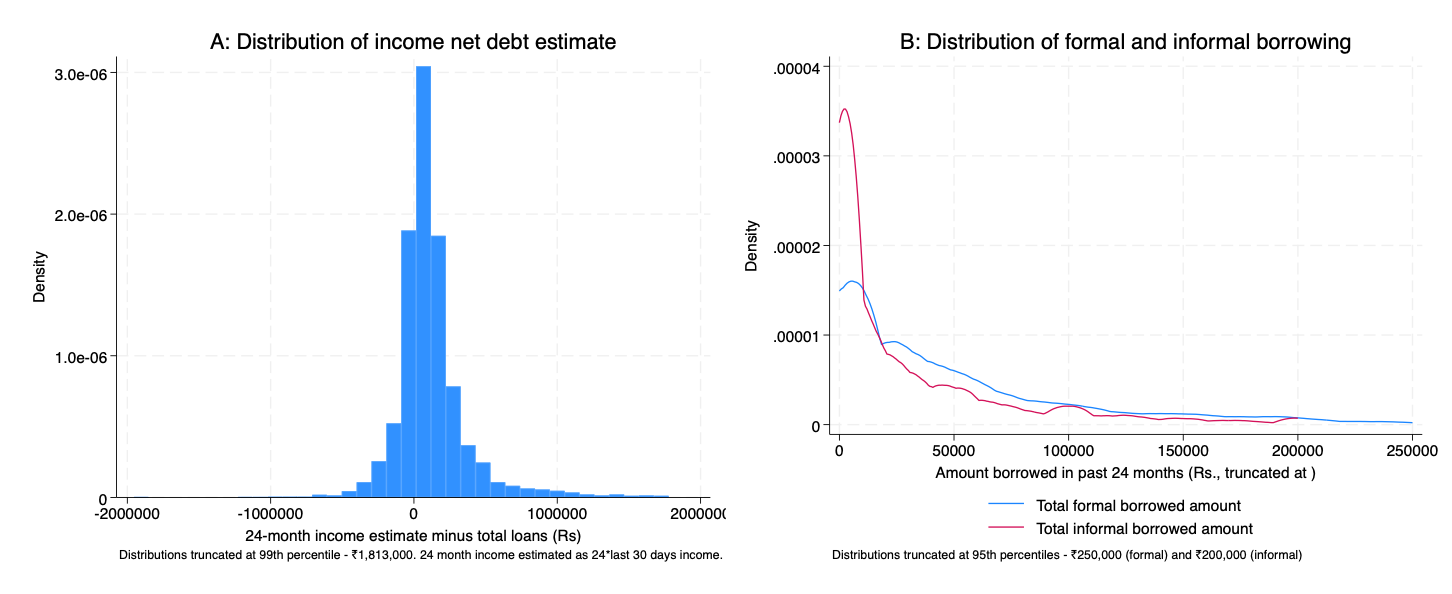
\includegraphics[width=\textwidth]{figures/figure02_loandistribution.png}
    \caption{: Distribution of total borrowing (loans) in last 24 months}
\end{figure}

Here we can see that informal borrowing is much more common


\subsection{part f}

top code so that upper end of the distribution is censored

large outliers skew stuff
might be measurement error or self reported bias or recall bias

check for extreme debt to income ratios 


\subsection{part j}

strengths of the dummy
- per-capita


weaknesses of the dummy
- ask about expenses to build local poverty line, perhaps nutrition based



\subsection{part k}

drop all baseline only - not even part of experiment

endline only not significantly different by treated or control

\section{part 2: analysis}

\subsection{part a}

testable hypothesis about impacts of the program on an outcome or subgroup

Early expansion of banks increased total formal borrowing among sc/st households less than other households

\subsection{part b}

Why did you choose these particular variables to test?

What are the results of the test, and what can they tell us about the validity of the
experiment?




\begin{table}[H]
    \centering
    \scriptsize % shrink text
    \setlength{\tabcolsep}{2pt}
    \renewcommand{\arraystretch}{2}
    \resizebox{\textwidth}{!}{{
\def\sym#1{\ifmmode^{#1}\else\(^{#1}\)\fi}
\begin{tabular}{l*{1}{cccc}}
\hline\hline
                    &\multicolumn{4}{c}{}                                        \\
                    &     Control&     Treated&  Difference         &          SE\\
\hline
\textbf{Demographics of head of household}&            &            &                     &            \\
Male                &       0.736&       0.720&       0.016         &     (0.014)\\
Age                 &      46.441&      47.059&      -0.618         &     (0.407)\\
\textbf{Highest education level of head of household}&            &            &                     &            \\
Able to read and write&       0.617&       0.620&      -0.004         &     (0.016)\\
No formal education &       0.221&       0.238&      -0.016         &     (0.014)\\
Primary (classes 1-5)&       0.319&       0.306&       0.013         &     (0.015)\\
classes 8-13        &       0.422&       0.402&       0.019         &     (0.016)\\
Graduate/Postgraduate/Vocational/Industrial diploma&       0.038&       0.054&      -0.016\sym{**} &     (0.007)\\
\textbf{Household size and composition}&            &            &                     &            \\
No of household members 18yo+&       3.172&       3.135&       0.037         &     (0.045)\\
No of household members <18yo&       1.430&       1.340&       0.090\sym{**} &     (0.040)\\
\textbf{Religion and caste/tribe of household}&            &            &                     &            \\
Muslim              &       0.033&       0.021&       0.012\sym{**} &     (0.005)\\
Christian           &       0.061&       0.039&       0.022\sym{***}&     (0.007)\\
Forward Caste       &       0.005&       0.008&      -0.003         &     (0.003)\\
Backward Caste      &       0.418&       0.373&       0.045\sym{***}&     (0.016)\\
Most Backward Caste &       0.316&       0.361&      -0.046\sym{***}&     (0.015)\\
Scheduled Caste and Tribe&       0.261&       0.258&       0.004         &     (0.014)\\
\hline
Observations        &        3802&            &                     &            \\
\hline\hline
\end{tabular}
}
}
    \caption{: Endline raw data summary statistics}
\end{table}


I chose to balance test the following variables because they might vary systematically by village, which is the unit of treatment assignment. If treatment assignment isn't effectively random, then the effect of local bank branches opening might be confounded with these variables. 

\begin{itemize}
    \item household head's gender, for instance, may be dependent on male/female preferring migration patterns that vary by village.

    \item household head's age, for instance, may be dependent on household structure norms that vary by village - if some communities remain in joint households after marriage, then household heads would likely be older. 

    \item similarly, the household size and composition variables may be correlated with structure norms that differ systematically by village.
    
    \item Indian villages often differ by social group composition, some may be mixed caste and religion, others may be more homogenous. Caste and religion, both individually and in village composition, is a strong determinant of health and socioeconomic outcomes in India.
    
\end{itemize}


\section{References used}

\end{document}
